\chapter{Marco teórico}

\section{Modelo estándar de partículas elementales}

El modelo estándar de física de partículas elementales (SM) es la teoría más exitosa jamás concebida, ha explicado con éxito casi todos los resultados experimentales y ha predicho con alta precisión una amplia variedad de fenómenos. Con el tiempo y a través de muchos experimentos, el SM se ha consolidado como la teoría física mejor probada. Esta teoría describe al universo al nivel más fundamental hasta hoy conocido, esto por medio de tres de las cuatro interacciones fundamentales de la naturaleza (nuclear fuerte, nuclear débil y electromagnética) y su forma de interactuar con quarks y leptones, donde los bosones de norma son los mediadores de dichas interacciones. El SM es una teoría cuántica de campos en la cual su Lagrangiano describe toda la cinemática y dinámica de la misma, donde las partículas son las excitaciones de los diferentes campos (cuantos). La  teoría está enmarcada dentro una simetría global, la simetría de Poincaré y una simetría local de norma (gauge) que básicamente define al SM, la simetría \(SU(3)_{C}\times SU(2)_{L}\times U(1)_{Y}\). Cabe resaltar que el SM depende de 19 parámetros para describir la dinámica, dichos parámetros cuentan con valores numéricos bien definidos y verificados experimentalmente.

La formulación actual del SM fue finalizada en los años 70’s luego de la contribución de muchos científicos con ideas revolucionarias como las de Gell-Mann y Zweig (\cite{GellMann:1964nj}, \cite{Zweig:1981pd}) en 1964 donde hacían referencia a que los hadrones son partículas compuestas por unas más fundamentales que denominaron quarks y sus antipartículas, los antiquarks. También, otra idea relevante y que además sería fuente de inspiración para Gell-Mann en el “camino del octete” es la existencia de las simetrías de gauge o simetrías locales, en este punto fueron especialmente importantes los aportes de Yang y Mills en 1954 \cite{PhysRev.96.191} para la construcción de una teoría de gauge basada en el grupo unidimensional \(U(1)\) de electrodinámica y el grupo tridimensional \(SU(2)\) de isospín, esta teoría era de basta elegancia, porque la simetría dictaba la forma de las interacciones. Pero no todo fue perfecto, ya que la teoría de Yang y Mills presentaba un inconveniente respecto a la masa de los bosones, la simetría de gauge prohíbe a los bosones de gauge tener masa, lo que promovía el insertar masas a mano y esto hacía a la teoría menos predictiva; este problema se soluciona con otra gran idea, el rompimiento espontáneo de simetría, este fue uno de los puntos cúspides en el desarrollo del SM y es allí donde Higgs en 1964 trabajó sobre las ideas originales de Yang y Mills considerando una simetría de gauge como la simetría de isospín local donde conservaría un bosón de Goldstone que se convierte en la parte de helicidad cero de un bosón de gauge con masa, este sería posteriormente conocido como el bosón de Higgs. 

Tenemos como componentes del SM dos teorías de gran calibre, la teoría electrodébil (EW) y la cromodinámica cuántica (QCD). La primera de ellas, la teoría electrodébil o también conocida como la teoría de Glashow-Weinberg-Salam (GWS) es una teoría de unificación que unió a la interacción débil con la interacción electromagnética. El planteamiento inicial de la teoría electrodébil fue propuesto por Glashow que enmarca dicha unión dentro de la simetría \(SU(2)\times U(1)\) (simetrías de isospín y electromagnética), mientras que por su parte Weinberg y Salam complementaron dicha teoría con base en el mecanismo de Higgs y cómo este dota de masa a las partículas de gauge y fermiones. QCD por otra parte es una teoría de norma basada en la simetría de color \(SU(3)\), esta teoría fue ideada con ayuda de los planteamientos hechos por Gell-Mann, Nishijima, Ne'eman, Zweig, Sakata, entre otros. Hasta llegar a la consolidación con las propuestas sobre la libertad asintótica de Gross y Wilczek, y de manera independiente por Politzer. QCD propone que los quarks pueden tener tres tipos de carga de color y que estos son la fuente de la interacción fuerte, mediada por los gluones que existen en 8 tipos. Las dos teorías mencionadas anteriormente son las que conforman a la teoría más exitosa jamás creada, el modelo estándar de física de partículas elementales. 
Ambas teorías, EW y QCD contienen la esencia del SM y lo podrían resumir de la siguiente manera: Los bloques de los cuales está hecha la materia son los quarks y leptones, sus interacciones están descritas dentro del marco matemático de las teorías de campo de norma y el vacío está en una especie de fase superconductora \cite{nagashima2013elementary}.

El SM contiene 12 fermiones compuestos por 6 leptones y 6 quarks. Cada clasificación se agrupa en pares, que forman tres generaciones o familias que se organizan en orden de masa creciente (ver figura \ref{fig:intro1}). Otra característica de la primera familia es que las partículas no se descomponen y además conforman toda la materia visible del universo, ya que es con partículas de esta familia que se forman los átomos. Ninguno de los neutrinos se descompone. Todos los bosones de gauge tienen espín 1 y, por lo tanto, no tienen que obedecer el principio de exclusión de Pauli. 

\begin{figure}[h]
    \centering
    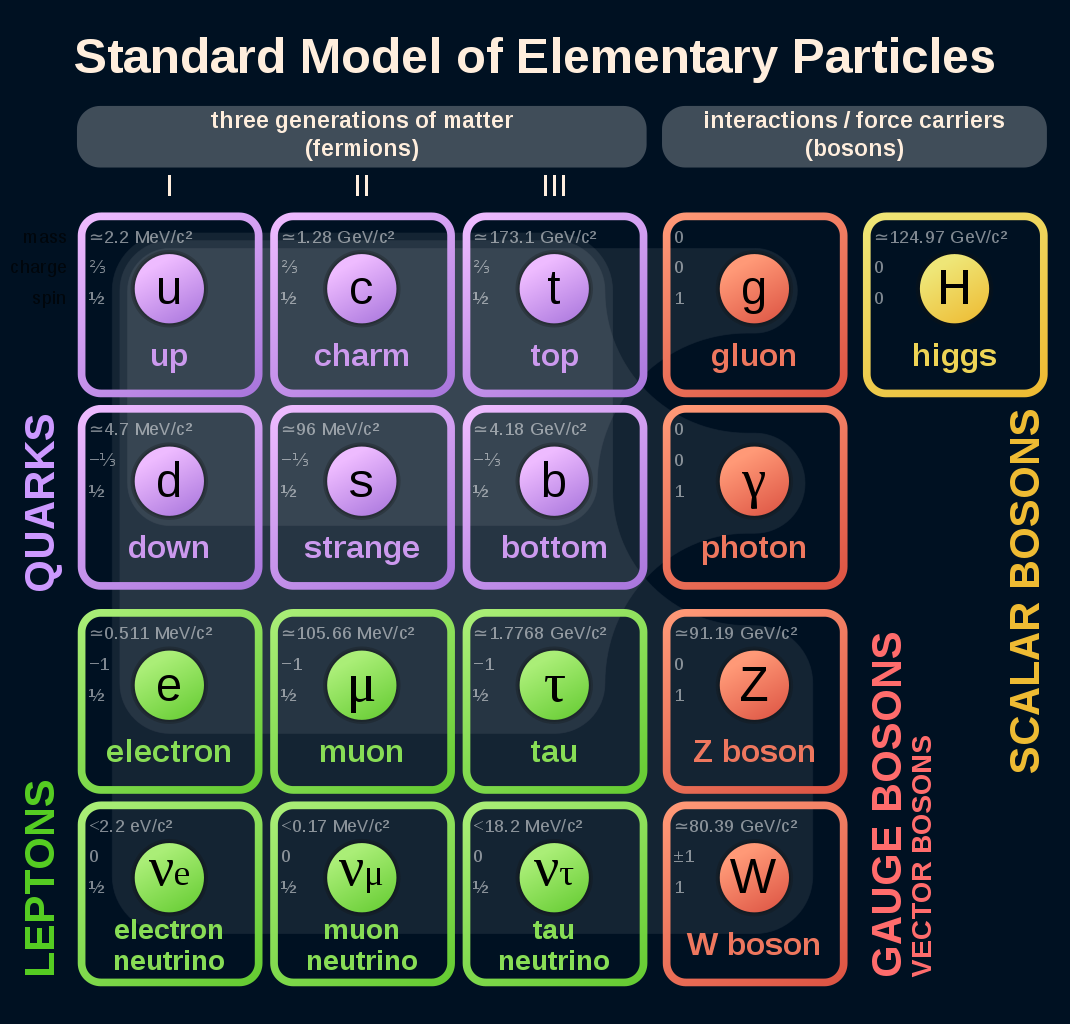
\includegraphics[scale=.25]{Images/1070px-Standard_Model_of_Elementary_Particles_dark.svg.png}
    \caption{\small Componentes del modelo estándar de partículas elementales}
    \label{fig:intro1}
\end{figure}

En el bloque de la izquierda de la figura \ref{fig:intro1} tenemos las tres generaciones que lo componen, los fermiones. Los fermiones son partículas de espín semientero y su dinámica proviene del Lagrangiano de Dirac,
\begin{equation}
    \mathcal{L} = \bar{\psi}\left(i\slashed \partial - m\right)\psi, \label{ladirac}
\end{equation}
donde \(\psi\) es el espinor de Dirac, \(\bar{\psi}=\psi^\dagger\gamma^0\) es su adjunto de Dirac, \(\gamma^0\) es una de las matrices gamma \(\gamma^\mu\) y \(\slashed\partial\) es la notación de slash de Feynman para \(\gamma^\mu\partial_{\mu}\). Con el Lagrangiano \ref{ladirac} se llega a la ecuación de Dirac, ecuación que gobierna la dinámica de los fermiones, originalmente en la solución de esta ecuación se llegó a una especie de paradoja en el espectro, ya que al solucionar el problema de la densidad de probabilidad Dirac le tuvo que dar una interpretación a las energías negativas que obtuvo, es por esto que planteó que el vacío también estaba ocupado. Es decir, ``Dirac esquivó las soluciones negativas de energía por invocación del principio de exlusión de Pauli (es así como esta ecuación describe a los fermiones). Él postuló que todas las energías están ocupadas y considerando al vacío como un mar infinito de electrones con \(E<0\).'' - \textit{Halzen} \cite{Halzen:1984mc}. La ausencia de un un fermión con carga negativa \(-e\) y energía \(-E\) es interpretado como la presencia de una antipartícula (antifermión) de carga \(+e\) y energía \(+E\). Feynman le daría otra interpretación para sus diagramas, donde plantea que las soluciones de energía negativa describen a una partícula la cual se propaga atrás en el tiempo o, equivalentemente una antipartícula con energía positiva propagándose adelante en el tiempo.

Por último, en la parte de la derecha de la figura \ref{fig:intro1} tenemos a los bosones, que se dividen en bosones de gauge y bosón escalar. Dentro de los bosones de norma tenemos a los bosones \(Z^0\) y \(W^{\pm}\) que son los responsables de mediar la interacción débil, también está el fotón que media la interacción electromagnética, los gluones que son los responsbles de la interacción fuerte y por último un bosón escalar, el bosón de Higgs que se encarga del mecanismo de Higgs que dota de masa a fermiones y partículas de gauge.

Como ya se ha mencionado el SM es una teoría de gauge, lo que quiere decir que su Lagrangiano \(\mathcal{L}_{SM}=\mathcal{L}(\psi,\partial_{\mu}\psi)\) permanece invariante bajo transformaciones de norma locales, del tipo \(\psi\rightarrow e^{-i\Lambda(x^\mu)}\psi\). Esta teoría está basada en el grupo de norma \(G=SU(3)\times SU(2)\times U(1)\), donde el factor electrodébil \(SU(2)\times U(1)\) es quiral, es decir que los fermiones izquierdos tienen cargas diferentes a las de los fermiones derechos. Esta es una de las razones por las cuales se requiere del mecanismo de Higgs para romper parte de la simetría de norma y permitir que el electrón y otros fermiones tengan masa. Por otra parte la simetría \(SU(3)\) (QCD) cuyo factor de norma es \(g_{s}\) que además contiene 8 bosones de gauge (gluones) es quiral. 

Debido a que el SM es una teoría cuántica de campos, las entidades que describen a las partículas son los campos cuánticos, los cuales están definidos para cada punto del espacio-tiempo y en este caso son los siguientes

\begin{itemize}
    \item el campo fermiónico, \(\psi\), que toma en cuenta a las partículas masivas;
    \item campos bosónicos electrodébiles, \(W_{1}\), \(W_{2}\), \(W_{3}\) y \(B\);
    \item el campo gluónico, \(G_{\alpha}\), y
    \item el campo de Higgs, \(\phi\).
\end{itemize}

La densidad Lagrangiana del SM es
\begin{equation}
    \mathcal{L}_{SM} = \mathcal{L}_{gauge}+\mathcal{L}_f+\mathcal{L}_\phi+\mathcal{L}_{Yuk},
\end{equation}
donde \(\mathcal{L}_{gauge}\) es el término de norma, \(\mathcal{L}_f\) el fermiónico, \(\mathcal{L}_\phi\) el Higgs y \(\mathcal{L}_{Yuk}\) el de Yukawa. Los términos de la parte de norma son
\begin{equation}
    \mathcal{L}_{gauge}=-\frac{1}{4}G^i_{\mu\nu}G^{\mu\nu i}-\frac{1}{4}W^i_{\mu\nu}W^{\mu\nu i}-\frac{1}{4}B_{\mu\nu}B^{\mu\nu} \label{lgauge}
\end{equation}
Aquí se incluye la energía cinética de los términos de bosones de norma, así como las autointeracciones de color y electrodébiles. Remarcamos que los tres tensores de intensidad de campo para \(SU(3)\), \(SU(2)\) y \(U(1)\) son respectivamente
\begin{eqnarray}
    G^i_{\mu\nu} &=& \partial_{\mu}G^i_{\nu}-\partial_{\nu}G^i_{\mu}-g_{s}f_{ijk}G^j_{k}G^i_{\nu},  \quad \textrm{i,j,k}=1...8 \nonumber \\
    W^i_{\mu\nu}&=&\partial_{\mu}W^i_{\nu}-\partial_{\nu}W^i_{\mu}-g\epsilon_{ijk}W^j_{\mu}W^k_{\nu},\quad \textrm{i,j,k}=1...3 \nonumber \\
    B_{\mu\nu} &=& \partial_{\nmu}B_{\nu}-\partial_{\nu}B_{\mu}.
\end{eqnarray}
\(\epsilon_{ijk}\) es el símbolo de Levi-Civita que indica las permutaciones y \(f_{ijk}\) es la constante de estructura del grupo de Lie \(SU(3)\) que es totalmente antisimétrica.

Para el término fermiónico tenemos que el sector electrodébil interactúa con el grupo de simetría \(SU(2)_L\times U(1)_{Y}\), donde el índice L indica el acople sólo con los fermiones izquierdos y \(Y\) la hipercarga, la densidad Lagrangiana electrodébil sería
\begin{equation}
    \mathcal{L}_{EW} = \sum_{\psi}^{F}\bar{\psi}\gamma^{\mu}\left(i\partial_{\mu}-\frac{1}{2}g'Y_{W}B_{\mu}-\frac{1}{2}\tau W_{\mu}\right)\psi, 
\end{equation}
donde la suma corre sobre F=3 familias, \(g'\) es el acople para \(U(1)\), \(g\) el de \(SU(2)\), \(Y_{W}\) es la hipercarga débil, \(B_{\mu}\) es el generador de grupo para \(U(1)\), mientras que \(W_{\mu}\) representa las tres componentes del campo de gauge para \(SU(2)\) Y \(\tau\) tiene como componentes las matrices de Pauli cuyos eigenvalores dan el isospín débil.

En adición, debemos contar con la contribución de QCD que sería
\begin{equation}
    \mathcal{L}_{QCD} = i\bar{U}\left(\partial_{\mu}-ig_{s}G^a_{\mu}T^a\right)\gamma^{\mu}U+i\bar{D}\left(\partial_{\mu}-ig_{s}G^a_{\mu}T^a\right)\gamma^\mu D, \label{lqcd}
\end{equation}
la anterior Lagrangiana define la interacción existente entre quarks y los gluones, cuya simetría como ya se ha mencionado es \(SU(3)\) y donde su generador es \(T^a\). Lo que tenemos en \ref{lqcd} es el lagrangiano de Dirac como en \ref{ladirac}, pero, en este caso se tiene quarks acoplados con campos gluónicos, donde \(U\) y \(D\) son los espinores para quarks up y down respectivamente.

Por último se debe considerar el mecanismo de Higgs, en esta parte se manifiestan tanto la Lagrangiana de Higgs como la interacción de Yukawa. La densidad Lagrangiana de Higgs es 
\begin{equation}
    \mathcal{L}_{\phi} = \left(D^\mu \phi\right)^2D_{\mu}\phi-V(\phi),
\end{equation}
donde \(D^{\mu}\) es la derivada covariante de gauge y el potencial de Higgs \(V(\phi)\) es el máxime responsable en el rompimiento espontáneo de la simetría y tiene la forma siguiente,
\begin{equation}
    V(\phi) = V(0)+\mu^2|\phi|^2+\lambda|\phi|^4, \quad |\phi| = \sqrt{|\phi^+|^2+|\phi^0|^2}
\end{equation}
\(V(0)\) es arbitraria y generalmente se asume un valor que haga desaparecer la energía del vacío, \(\mu\) representa la masa del cuanto y el término \(\lambda\) representa la interacción entre campos de Higgs. Por su parte el campo \(\phi\) se puede escribir como: 
\begin{align}
    \phi &= \frac{1}{\sqrt{2}} \begin{pmatrix}
           \phi^+ \\
           \phi^0 \\
         \end{pmatrix},
\end{align}
se resalta que los superíndices + y 0 indican la carga (Q) de las componentes. Por su parte la hipercarga \(Y_{W}\) es 1 para ambas componentes.
La interacción de Yukawa se evidencia en el término
\begin{equation}
    \mathcal{L}_{Yuk} = \bar{U}_{L}G_{u}U_{R}\phi^0-\bar{D}_{L}G_{u}U_{R}\phi^- +\bar{U}_{L}G_{d}D_{R}\phi^{+}+ \bar{D}_{L}G_{d}D_{R}\phi^0 +h.c,
\end{equation}
donde los \(G_{u,d}\) son los acoples de Yukawa.

\section{Leptón tau}

El leptón tau es el leptón más masivo de las tres familias, su gran masa de aproximadamente 1777 MeV, unas 3477 veces más masivo que el electrón y unas 17 veces más pesado que el muón. Esta
cualidad lo hace interesante para poner a prueba el Modelo Estándar de partículas, en búsqueda de nueva física, estudios de violación de sabor leptónico, universalidad leptónica, pruebas de CPT. Lo anterior ha hecho suponer que el tau podría no ser una partícula fundamental, es decir, que estuviese compuesta por un tipo de constituyentes similares a los quarks, se les llama lepto-quarks, pero hasta el momento es solo eso, una suposición. Lo que sí está ampliamente validado es que el leptón tau gracias  a su enorme masa cuenta con una gran cantidad de canales de decaimiento, además de ser el único leptón capaz de decaer en hadrones. El tercer leptón fue descubierto por Martin Lewis Perl, \textit{et al.} en 1975 y confirmado por múltiples experimentos como SLAC, DORIS, DESY, entre otros. La historia del descubrimiento del tau se sintetiza en el review \cite{Perl_1992}.

El tau genera muchas expectativas entorno suyo, ya que debido a sus múltiples canales de decaimiento, su gran masa y su corto tiempo de vida (\(\sim3\times10^{-13}s\)), hace que esta partícula sea sensible a la nueva física (NP) o física más allá del modelo estándar (BSM), han habido indicios de esto, uno en particular es en estudios referentes al momento dipolar eléctrico (EDM), medición realizada por la colaboración Belle \cite{Inami_2003}. Un valor diferente de cero del EDM podría indicar violación de carga-paridad (CPV), llevándonos nuevamente a indicios de NP ya que BSM puede producir CPV en procesos leptónicos. El experimento Belle II en el SuperKEKB es el mejor lugar para estudiar EDM porque sus actualizaciones han logrado un récord de luminosidad que implica más estadística y sensibilidad, por estas razones se puede obtener una mejor medición de EDM del leptón tau. 
Otro proceso interesante de medir en el leptón tau es la violación carga-paridad-tiempo (CPT), que en el SM debe ser conservada en su totalidad. Esto puede testearse en la diferencia de masa entre \(\tau^-\) y \(\tau^+\), ya que una diferencia en la masa de estos podría representar una no conservación de CPT. Ambas mediciones fueron realizadas por Belle \cite{PhysRevLett.99.011801} en 2007 y se planean realizar en Belle II. 